\documentclass[aspectratio=169]{beamer}
\usepackage{graphicx}
\usepackage{amsmath}
\usepackage{amssymb}
\usepackage{tikz}
% \usepackage{algorithm}
% \usepackage{algorithmic}
\usepackage[linesnumbered,ruled,vlined]{algorithm2e}
\usepackage{xcolor}
\usepackage{booktabs}
\usepackage{subcaption}
\usepackage{animate}
\usepackage{hyperref}


\usepackage{amsmath}

\DeclareMathOperator*{\argmax}{arg\,max}

% Theme and color scheme
\usetheme{Madrid}
\usecolortheme{default}

% Custom colors
\definecolor{darkblue}{RGB}{0,51,102}
\definecolor{lightblue}{RGB}{173,216,230}
\definecolor{green}{RGB}{0,128,0}
\definecolor{red}{RGB}{220,20,60}

\title[Q-Learning Grid World]{Q-Learning in Grid World Environment}
\subtitle{Team 09 - Homework 1}
\author[Team 09]{Shayan Meshkat Alsadat}
\institute[ASU]{Reinforcement Learning in Robotics}
\date{\today}

\begin{document}

% Title slide
\begin{frame}
    \titlepage
\end{frame}

% Outline
\begin{frame}{Outline}
    \tableofcontents
\end{frame}

\section{Introduction and Environment Setup}

\begin{frame}{Grid World Environment}
    \begin{columns}
        \begin{column}{0.5\textwidth}
            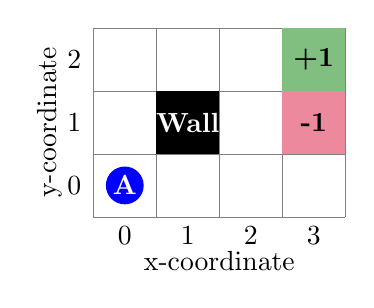
\begin{tikzpicture}[scale=0.8]
                % Grid
                \draw[step=1cm,gray,very thin] (0,0) grid (4,3);
                
                % Walls
                \fill[black] (1,1) rectangle (2,2);
                \node at (1.5,1.5) {\color{white}\textbf{Wall}};
                
                % Goal
                \fill[green!50] (3,2) rectangle (4,3);
                \node at (3.5,2.5) {\textbf{+1}};
                
                % Penalty
                \fill[red!50] (3,1) rectangle (4,2);
                \node at (3.5,1.5) {\textbf{-1}};
                
                % Starting position
                \fill[blue] (0.5,0.5) circle (0.3);
                \node at (0.5,0.5) {\color{white}\textbf{A}};
                 
                        % Grid labels
                        \foreach \x in {0,1,2,3}
                            \node at (\x+0.5,-0.3) {\x};
                        \foreach \y in {0,1,2}
                            \node at (-0.3,\y+0.5) {\y};
                    
                \node at (2,-0.7) {x-coordinate};
                \node[rotate=90] at (-0.7,1.5) {y-coordinate};
            \end{tikzpicture}
        \end{column}
        \begin{column}{0.5\textwidth}
            \textbf{Environment Specifications:}
            \begin{itemize}
                \item \textbf{Grid Size:} $4 \times 3$
                \item \textbf{Starting Position for Agent:} $(0,0)$
                \item \textbf{Goal:} $(3,2)$ with reward $+1$
                \item \textbf{Penalty:} $(3,1)$ with reward $-1$ or $-100$
                \item \textbf{Wall:} $(1,1)$ - blocked
                \item \textbf{Step Cost:} $-0.04$ per move
            \end{itemize}
            
            \vspace{0.5cm}
            \textbf{Action Space:}
            \begin{itemize}
                \item Up, Down, Left, Right
                \item Slip mechanics: $80\%$ intended, $10\%$ left, $10\%$ right
            \end{itemize}
        \end{column}
    \end{columns}
\end{frame}

\section{Q-Learning Algorithm}

\begin{frame}{Q-Learning Algorithm}
    \begin{columns}
        \begin{column}{0.5\textwidth}
            \begin{algorithm}[H]
                \caption{Q-Learning Algorithm}
                \SetAlgoLined
                \small
                Initialize $Q(s,a) = 0 \ \forall \  s \in S,a \in A$, $N$ steps\;
                \For{each episode}{
                    Initialize state $s = s_{0} \in S$\;
                    \While{$s \neq (3,2) \vee s \neq (3, 1) \vee i \leq N$}{
                        $\rho \gets \text{random number in } [0,1]$\;
                        \eIf{$\rho < \epsilon$}{
                            Choose random action $a \in A$\;
                        }{
                             $a \gets \argmax_{a \in A} Q(s,a)$\;
                        }
                        $s^{\prime} \gets \text{take action } a$, $ r \gets \text{receive reward}$\;
                        Update: $Q(s,a) \leftarrow Q(s,a) + \alpha[r + \gamma \max_{a'}Q(s',a') - Q(s,a)]$\;
                        $s \leftarrow s'$, $i \leftarrow i + 1$\;
                    }
                }
            \end{algorithm}
        \end{column}
        \begin{column}{0.4\textwidth}
            \textbf{Hyperparameters:}
            \begin{itemize}
                \item Learning rate: $\alpha = 0.01$
                \item Discount factor: $\gamma = 0.9$
                \item Exploration rate: $\epsilon = 0.1$
                \item Max steps: 80
                \item Training episodes: 5000
                \item Test episodes: 1000
            \end{itemize}
        \end{column}
    \end{columns}
\end{frame}

\begin{frame}{Q-Value Update Example - Step 1}
    
    \begin{columns}
        \begin{column}{0.45\textwidth}
            \textbf{Initial Q-Table (All Zeros)}
            \small
            \begin{table}[h]
                \centering
                \begin{tabular}{|c|c|c|c|c|}
                    \hline
                    \textbf{State} & \textbf{Up} & \textbf{Down} & \textbf{Left} & \textbf{Right} \\
                    \hline
                    (0,0) & 0.000 & 0.000 & 0.000 & 0.000 \\
                    (1,0) & 0.000 & 0.000 & 0.000 & 0.000 \\
                    (2,0) & 0.000 & 0.000 & 0.000 & 0.000 \\
                    (3,0) & 0.000 & 0.000 & 0.000 & 0.000 \\
                    \dots & \dots & \dots & \dots & \dots \\
                    \hline
                \end{tabular}
            \end{table}
            
            \textbf{Parameters:}
            \begin{itemize}
                \item $\alpha = 0.1$ (learning rate)
                \item $\gamma = 0.9$ (discount factor)
                \item $\epsilon = 0.1$ (exploration rate), Step cost: $r = -0.04$
            \end{itemize}
        \end{column}
        
        \begin{column}{0.55\textwidth}
            \textbf{Epsilon-Greedy Action Selection:}
            
            \textbf{Step 1: Generate random number}
            $$\rho \gets \text{uniform random number in } [0,1] = 0.85 $$
            
            \textbf{Step 2: Action selection} \\
            \eIf{$\rho = 0.85 < \epsilon = 0.1$}{
                Choose random action $a \in A$
            }{
                $a \gets \argmax_{a \in A} Q(s,a) = \argmax_{a \in A} Q((0,0), a) = \argmax_{a \in A} \{0, 0, 0, 0\}$
            }
            
            \textbf{Since all Q-values are 0:}
            \begin{itemize}
                \item All actions have equal Q-value
                \item Tie-breaking: choose randomly among best $\rightarrow$ \textbf{Selected action: Right} (random choice)
            \end{itemize}
        \end{column}
    \end{columns}
\end{frame}

\begin{frame}{Q-Value Update Example - Step 1 (continued)}
   
    
    \begin{columns}
        \begin{column}{0.5\textwidth}
            \textbf{Q-Table Before Update}
            \small
            \begin{table}[h]
                \centering
                \begin{tabular}{|c|c|c|c|c|}
                    \hline
                    \textbf{State} & \textbf{Up} & \textbf{Down} & \textbf{Left} & \textbf{Right} \\
                    \hline
                    (0,0) & 0.000 & 0.000 & 0.000 & 0.000 \\
                    (1,0) & 0.000 & 0.000 & 0.000 & 0.000 \\
                    (2,0) & 0.000 & 0.000 & 0.000 & 0.000 \\
                    (3,0) & 0.000 & 0.000 & 0.000 & 0.000 \\
                    \dots & \dots & \dots & \dots & \dots \\
                    \hline
                \end{tabular}
            \end{table}
            
            \textbf{Q-Table After Update}
            \small
            \begin{table}[h]
                \centering
                \begin{tabular}{|c|c|c|c|c|}
                    \hline
                    \textbf{State} & \textbf{Up} & \textbf{Down} & \textbf{Left} & \textbf{Right} \\
                    \hline
                    (0,0) & 0.000 & 0.000 & 0.000 & \textcolor{red}{-0.004} \\
                    (1,0) & 0.000 & 0.000 & 0.000 & 0.000 \\
                    (2,0) & 0.000 & 0.000 & 0.000 & 0.000 \\
                    (3,0) & 0.000 & 0.000 & 0.000 & 0.000 \\
                    \dots & \dots & \dots & \dots & \dots \\
                    \hline
                \end{tabular}
            \end{table}
        \end{column}
        
        \begin{column}{0.5\textwidth}
            \textbf{Update Formula:}
            $$Q(s,a) \leftarrow Q(s,a) + \alpha[r + \gamma \max_{a'}Q(s',a') - Q(s,a)]$$
            
          
            \begin{align}
                s &= (0,0), \quad a = \text{Right} \\
                s' &= (1,0), \quad r = -0.04 \\
                \max_{a'}Q(s',a') &= 0 \\
                Q((0,0),\text{Right}) &= 0 + 0.1[-0.04 + 0.9 \cdot 0 - 0] \\
                &= \textcolor{red}{-0.004}
            \end{align}
            
           
            \textbf{Current State:} Agent moves to (1,0)
        \end{column}
    \end{columns}
\end{frame}

\begin{frame}{Q-Value Update Example - Step 2}
    
    \begin{columns}
        \begin{column}{0.45\textwidth}
            \textbf{Q-Table}
            \small
            \begin{table}[h]
                \centering
                \begin{tabular}{|c|c|c|c|c|}
                    \hline
                    \textbf{State} & \textbf{Up} & \textbf{Down} & \textbf{Left} & \textbf{Right} \\
                    \hline
                    (0,0) & 0.000 & 0.000 & 0.000 & \textcolor{red}{-0.004} \\
                    (1,0) & 0.000 & 0.000 & 0.000 & 0.000 \\
                    (2,0) & 0.000 & 0.000 & 0.000 & 0.000 \\
                    (3,0) & 0.000 & 0.000 & 0.000 & 0.000 \\
                    \dots & \dots & \dots & \dots & \dots \\
                    \hline
                \end{tabular}
            \end{table}
            
            \textbf{Current State:} Agent at (1,0)
            
            \vspace{0.3cm}
            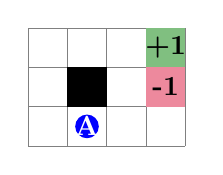
\begin{tikzpicture}[scale=0.5]
                % Grid
                \draw[step=1cm,gray,very thin] (0,0) grid (4,3);
                
                % Walls
                \fill[black] (1,1) rectangle (2,2);
                
                % Goal
                \fill[green!50] (3,2) rectangle (4,3);
                \node at (3.5,2.5) {\textbf{+1}};
                
                % Penalty
                \fill[red!50] (3,1) rectangle (4,2);
                \node at (3.5,1.5) {\textbf{-1}};
                
                % Agent position
                \fill[blue] (1.5,0.5) circle (0.3);
                \node at (1.5,0.5) {\color{white}\textbf{A}};
            \end{tikzpicture}
        \end{column}
        
        \begin{column}{0.55\textwidth}
           
            
            
            $$\rho \gets \text{uniform random number in } [0,1] = 0.05 $$
            
            \textbf{Action selection:} \\ 
            \eIf{$\rho = 0.05 < \epsilon = 0.1$}{
                Choose random action $a \in A$ $\rightarrow$ \textbf{Selected: Up}
            }{
                $a \gets \argmax_{a \in A} Q((1,0), a) = \argmax_{a \in A} \{0, 0, 0, 0\}$
            }
            
            Agent randomly selects Up action
        \end{column}
    \end{columns}
\end{frame}

\begin{frame}{Q-Value Update Example - Step 2 (continued)}
 
    
    \begin{columns}
        \begin{column}{0.5\textwidth}
            \textbf{Q-Table Before Update}
            \small
            \begin{table}[h]
                \centering
                \begin{tabular}{|c|c|c|c|c|}
                    \hline
                    \textbf{State} & \textbf{Up} & \textbf{Down} & \textbf{Left} & \textbf{Right} \\
                    \hline
                    (0,0) & 0.000 & 0.000 & 0.000 & \textcolor{red}{-0.004} \\
                    (1,0) & 0.000 & 0.000 & 0.000 & 0.000 \\
                    (2,0) & 0.000 & 0.000 & 0.000 & 0.000 \\
                    (3,0) & 0.000 & 0.000 & 0.000 & 0.000 \\
                    \dots & \dots & \dots & \dots & \dots \\
                    \hline
                \end{tabular}
            \end{table}
            
            \textbf{Q-Table After Update}
            \small
            \begin{table}[h]
                \centering
                \begin{tabular}{|c|c|c|c|c|}
                    \hline
                    \textbf{State} & \textbf{Up} & \textbf{Down} & \textbf{Left} & \textbf{Right} \\
                    \hline
                    (0,0) & 0.000 & 0.000 & 0.000 & \textcolor{red}{-0.004} \\
                    (1,0) & \textcolor{blue}{-0.004} & 0.000 & 0.000 & 0.000 \\
                    (2,0) & 0.000 & 0.000 & 0.000 & 0.000 \\
                    (3,0) & 0.000 & 0.000 & 0.000 & 0.000 \\
                    \dots & \dots & \dots & \dots & \dots \\
                    \hline
                \end{tabular}
            \end{table}
        \end{column}
        
        \begin{column}{0.5\textwidth}
            
            \begin{align}
                s &= (1,0), \quad a = \text{Up} \\
                s' &= (1,0), \quad r = -0.04 \\
                \max_{a'}Q(s',a') &= 0 \\
                Q((1,0),\text{Up}) &= 0 + 0.1[-0.04 + 0.9 \cdot 0 - 0] \\
                &= \textcolor{blue}{-0.004}
            \end{align}
            
            \vspace{0.5cm}
            \textbf{Current State:} Agent stays at (1,0)
        \end{column}
    \end{columns}
\end{frame}







\begin{frame}{Q-Value Update Example - Step 3}
    
    \begin{columns}
        \begin{column}{0.45\textwidth}
            \textbf{Q-Table}
            \small
            \begin{table}[h]
                \centering
                \begin{tabular}{|c|c|c|c|c|}
                    \hline
                    \textbf{State} & \textbf{Up} & \textbf{Down} & \textbf{Left} & \textbf{Right} \\
                    \hline
                    (0,0) & 0.000 & 0.000 & 0.000 & \textcolor{red}{-0.004} \\
                    (1,0) & \textcolor{red}{-0.004} & 0.000 & 0.000 & 0.000 \\
                    (2,0) & 0.000 & 0.000 & 0.000 & 0.000 \\
                    (3,0) & 0.000 & 0.000 & 0.000 & 0.000 \\
                    \dots & \dots & \dots & \dots & \dots \\
                    \hline
                \end{tabular}
            \end{table}
            
            \textbf{Current State:} Agent at (1,0)

                        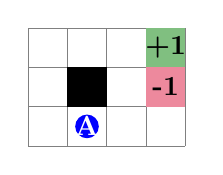
\begin{tikzpicture}[scale=0.5]
                % Grid
                \draw[step=1cm,gray,very thin] (0,0) grid (4,3);
                
                % Walls
                \fill[black] (1,1) rectangle (2,2);
                
                % Goal
                \fill[green!50] (3,2) rectangle (4,3);
                \node at (3.5,2.5) {\textbf{+1}};
                
                % Penalty
                \fill[red!50] (3,1) rectangle (4,2);
                \node at (3.5,1.5) {\textbf{-1}};
                
                % Agent position
                \fill[blue] (1.5,0.5) circle (0.3);
                \node at (1.5,0.5) {\color{white}\textbf{A}};
            \end{tikzpicture}

        \end{column}
        
        \begin{column}{0.55\textwidth}
            
            
            
            $$\rho \gets \text{uniform random number in } [0,1] = 0.08 $$
            
            \textbf{Action selection:} \\ 
            \eIf{$\rho = 0.08 < \epsilon = 0.1$}{
                Choose random action $a \in A$ $\rightarrow$ \textbf{Selected: Right}
            }{
                $a \gets \argmax_{a \in A} Q((1,0), a) = \argmax_{a \in A} \{0, 0, 0, 0\}$
            }

             Agent randomly selects Right action
        \end{column}
    \end{columns}
\end{frame}

\begin{frame}{Q-Value Update Example - Step 3 (continued)}
    
    \begin{columns}
        \begin{column}{0.5\textwidth}
            \textbf{Q-Table Before Update}
            \small
            \begin{table}[h]
                \centering
                \begin{tabular}{|c|c|c|c|c|}
                    \hline
                    \textbf{State} & \textbf{Up} & \textbf{Down} & \textbf{Left} & \textbf{Right} \\
                    \hline
                    (0,0) & 0.000 & 0.000 & 0.000 & \textcolor{red}{-0.004} \\
                    (1,0) & \textcolor{red}{-0.004} & 0.000 & 0.000 & 0.000 \\
                    (2,0) & 0.000 & 0.000 & 0.000 & 0.000 \\
                    (3,0) & 0.000 & 0.000 & 0.000 & 0.000 \\
                    \dots & \dots & \dots & \dots & \dots \\
                    \hline
                \end{tabular}
            \end{table}
            
            \textbf{Q-Table After Update}
            \small
            \begin{table}[h]
                \centering
                \begin{tabular}{|c|c|c|c|c|}
                    \hline
                    \textbf{State} & \textbf{Up} & \textbf{Down} & \textbf{Left} & \textbf{Right} \\
                    \hline
                    (0,0) & 0.000 & 0.000 & 0.000 & \textcolor{red}{-0.004} \\
                    (1,0) & \textcolor{red}{-0.004} & 0.000 & 0.000 & \textcolor{blue}{-0.004} \\
                    (2,0) & 0.000 & 0.000 & 0.000 & 0.000 \\
                    (3,0) & 0.000 & 0.000 & 0.000 & 0.000 \\
                    \dots & \dots & \dots & \dots & \dots \\
                    \hline
                \end{tabular}
            \end{table}
        \end{column}
        
        \begin{column}{0.5\textwidth}
            
            \begin{align}
                s &= (1,0), \quad a = \text{Right} \\
                s' &= (2,0), \quad r = -0.04 \\
                \max_{a'}Q(s',a') &= 0 \\
                Q((1,0),\text{Right}) &= 0 + 0.1[-0.04 + 0.9 \cdot 0 - 0] \\
                &= \textcolor{blue}{-0.004}
            \end{align}
            
            \vspace{0.5cm}
            \textbf{Current State:} Agent goes to (2,0)
        \end{column}
    \end{columns}
\end{frame}












\begin{frame}{Q-Value Update Example - Step 4}
    
    \begin{columns}
        \begin{column}{0.45\textwidth}
            \textbf{Q-Table}
            \small
            \begin{table}[h]
                \centering
                \begin{tabular}{|c|c|c|c|c|}
                    \hline
                    \textbf{State} & \textbf{Up} & \textbf{Down} & \textbf{Left} & \textbf{Right} \\
                    \hline
                    (0,0) & 0.000 & 0.000 & 0.000 & \textcolor{red}{-0.004} \\
                    (1,0) & \textcolor{red}{-0.004} & 0.000 & 0.000 & \textcolor{red}{-0.004} \\
                    (2,0) & 0.000 & 0.000 & 0.000 & 0.000 \\
                    (3,0) & 0.000 & 0.000 & 0.000 & 0.000 \\
                    \dots & \dots & \dots & \dots & \dots \\
                    \hline
                \end{tabular}
            \end{table}
            
            \textbf{Current State:} Agent at (2,0)

            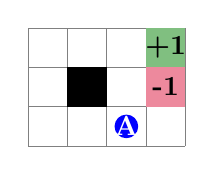
\begin{tikzpicture}[scale=0.5]
                % Grid
                \draw[step=1cm,gray,very thin] (0,0) grid (4,3);
                
                % Walls
                \fill[black] (1,1) rectangle (2,2);
                
                % Goal
                \fill[green!50] (3,2) rectangle (4,3);
                \node at (3.5,2.5) {\textbf{+1}};
                
                % Penalty
                \fill[red!50] (3,1) rectangle (4,2);
                \node at (3.5,1.5) {\textbf{-1}};
                
                % Agent position
                \fill[blue] (2.5,0.5) circle (0.3);
                \node at (2.5,0.5) {\color{white}\textbf{A}};
            \end{tikzpicture}

        \end{column}
        
        \begin{column}{0.55\textwidth}
            
            
            
            $$\rho \gets \text{uniform random number in } [0,1] = 0.5 $$
            
            \textbf{Action selection:} \\
            \eIf{$\rho = 0.5 < \epsilon = 0.1$}{
                Choose random action $a \in A$ $\rightarrow$
            }{
                $a \gets \argmax_{a \in A} Q((2,0), a) = \argmax_{a \in A} \{0, 0, 0, 0\}$
            }

             Tie break: agent randomly selects Down action
        \end{column}
    \end{columns}
\end{frame}

\begin{frame}{Q-Value Update Example - Step 4 (continued)}
    
    \begin{columns}
        \begin{column}{0.5\textwidth}
            \textbf{Q-Table Before Update}
            \small
            \begin{table}[h]
                \centering
                \begin{tabular}{|c|c|c|c|c|}
                    \hline
                    \textbf{State} & \textbf{Up} & \textbf{Down} & \textbf{Left} & \textbf{Right} \\
                    \hline
                    (0,0) & 0.000 & 0.000 & 0.000 & \textcolor{red}{-0.004} \\
                    (1,0) & \textcolor{red}{-0.004} & 0.000 & 0.000 & \textcolor{red}{-0.004} \\
                    (2,0) & 0.000 & 0.000 & 0.000 & 0.000 \\
                    (3,0) & 0.000 & 0.000 & 0.000 & 0.000 \\
                    \dots & \dots & \dots & \dots & \dots \\
                    \hline
                \end{tabular}
            \end{table}
            
            \textbf{Q-Table After Update}
            \small
            \begin{table}[h]
                \centering
                \begin{tabular}{|c|c|c|c|c|}
                    \hline
                    \textbf{State} & \textbf{Up} & \textbf{Down} & \textbf{Left} & \textbf{Right} \\
                    \hline
                    (0,0) & 0.000 & 0.000 & 0.000 & \textcolor{red}{-0.004} \\
                    (1,0) & \textcolor{red}{-0.004} & 0.000 & 0.000 & \textcolor{red}{-0.004} \\
                    (2,0) & 0.000 & \textcolor{blue}{-0.004} & 0.000 & 0.000 \\
                    (3,0) & 0.000 & 0.000 & 0.000 & 0.000 \\
                    \dots & \dots & \dots & \dots & \dots \\
                    \hline
                \end{tabular}
            \end{table}
        \end{column}
        
        \begin{column}{0.5\textwidth}
            
            \begin{align}
                s &= (2,0), \quad a = \text{Down} \\
                s' &= (3,0) \text{\textcolor{red}{slip}}, \quad r = -0.04 \\
                \max_{a'}Q(s',a') &= 0 \\
                Q((2,0),\text{Down}) &= 0 + 0.1[-0.04 + 0.9 \cdot 0 - 0] \\
                &= \textcolor{blue}{-0.004}
            \end{align}
            
            \vspace{0.5cm}
            \textbf{Current State:} Agent goes to $(3,0)$
        \end{column}
    \end{columns}
\end{frame}








\begin{frame}{Q-Value Update Example - Step 5}
    
    \begin{columns}
        \begin{column}{0.45\textwidth}
            \textbf{Q-Table After Update}
            \small
            \begin{table}[h]
                \centering
                \begin{tabular}{|c|c|c|c|c|}
                    \hline
                    \textbf{State} & \textbf{Up} & \textbf{Down} & \textbf{Left} & \textbf{Right} \\
                    \hline
                    (0,0) & 0.000 & 0.000 & 0.000 & \textcolor{red}{-0.004} \\
                    (1,0) & \textcolor{red}{-0.004} & 0.000 & 0.000 & \textcolor{red}{-0.004} \\
                    (2,0) & 0.000 & \textcolor{red}{-0.004} & 0.000 & 0.000 \\
                    (3,0) & 0.000 & 0.000 & 0.000 & 0.000 \\
                    \dots & \dots & \dots & \dots & \dots \\
                    \hline
                \end{tabular}
            \end{table}
            
            \textbf{Current State:} Agent at (3,0)

            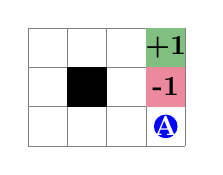
\begin{tikzpicture}[scale=0.5]
                % Grid
                \draw[step=1cm,gray,very thin] (0,0) grid (4,3);
                
                % Walls
                \fill[black] (1,1) rectangle (2,2);
                
                % Goal
                \fill[green!50] (3,2) rectangle (4,3);
                \node at (3.5,2.5) {\textbf{+1}};
                
                % Penalty
                \fill[red!50] (3,1) rectangle (4,2);
                \node at (3.5,1.5) {\textbf{-1}};
                
                % Agent position
                \fill[blue] (3.5,0.5) circle (0.3);
                \node at (3.5,0.5) {\color{white}\textbf{A}};
            \end{tikzpicture}

        \end{column}
        
        \begin{column}{0.55\textwidth}
            
            
            
            $$\rho \gets \text{uniform random number in } [0,1] = 0.7 $$
            
            \textbf{Action selection:} \\
            \eIf{$\rho = 0.7 < \epsilon = 0.1$}{
                Choose random action $a \in A$ $\rightarrow$
            }{
                $a \gets \argmax_{a \in A} Q((3,0), a) = \argmax_{a \in A} \{0, 0, 0, 0\}$
            }

             Tie break: agent randomly selects Left action
        \end{column}
    \end{columns}
\end{frame}

\begin{frame}{Q-Value Update Example - Step 5 (continued)}
    
    \begin{columns}
        \begin{column}{0.5\textwidth}
            \textbf{Q-Table Before Update}
            \small
            \begin{table}[h]
                \centering
                \begin{tabular}{|c|c|c|c|c|}
                    \hline
                    \textbf{State} & \textbf{Up} & \textbf{Down} & \textbf{Left} & \textbf{Right} \\
                    \hline
                    (0,0) & 0.000 & 0.000 & 0.000 & \textcolor{red}{-0.004} \\
                    (1,0) & \textcolor{red}{-0.004} & 0.000 & 0.000 & \textcolor{red}{-0.004} \\
                    (2,0) & 0.000 & \textcolor{red}{-0.004} & 0.000 & 0.000 \\
                    (3,0) & 0.000 & 0.000 & 0.000 & 0.000 \\
                    \dots & \dots & \dots & \dots & \dots \\
                    \hline
                \end{tabular}
            \end{table}
            
            \textbf{Q-Table After Update}
            \small
            \begin{table}[h]
                \centering
                \begin{tabular}{|c|c|c|c|c|}
                    \hline
                    \textbf{State} & \textbf{Up} & \textbf{Down} & \textbf{Left} & \textbf{Right} \\
                    \hline
                    (0,0) & 0.000 & 0.000 & 0.000 & \textcolor{red}{-0.004} \\
                    (1,0) & \textcolor{red}{-0.004} & 0.000 & 0.000 & \textcolor{red}{-0.004} \\
                    (2,0) & 0.000 & \textcolor{red}{-0.004} & 0.000 & 0.000 \\
                    (3,0) & 0.000 & 0.000 & \textcolor{blue}{-0.004} & 0.000 \\
                    \dots & \dots & \dots & \dots & \dots \\
                    \hline
                \end{tabular}
            \end{table}
        \end{column}
        
        \begin{column}{0.5\textwidth}
            
            \begin{align}
                s &= (3,0), \quad a = \text{Left} \\
                s' &= (2,0), \quad r = -0.04 \\
                \max_{a'}Q(s',a') &= 0 \\
                Q((3,0),\text{Left}) &= 0 + 0.1[-0.04 + 0.9 \cdot 0 - 0] \\
                &= \textcolor{blue}{-0.004}
            \end{align}
            
            \vspace{0.5cm}
            \textbf{Current State:} Agent goes to $(2,0)$
        \end{column}
    \end{columns}
\end{frame}



\begin{frame}{Q-Value Update Example - Step 6}
    
    \begin{columns}
        \begin{column}{0.45\textwidth}
            \textbf{Q-Table}
            \small
            \begin{table}[h]
                \centering
                \begin{tabular}{|c|c|c|c|c|}
                    \hline
                    \textbf{State} & \textbf{Up} & \textbf{Down} & \textbf{Left} & \textbf{Right} \\
                    \hline
                    (0,0) & 0.000 & 0.000 & 0.000 & \textcolor{red}{-0.004} \\
                    (1,0) & \textcolor{red}{-0.004} & 0.000 & 0.000 & \textcolor{red}{-0.004} \\
                    (2,0) & 0.000 & \textcolor{red}{-0.004} & 0.000 & 0.000 \\
                    (3,0) & 0.000 & 0.000 & \textcolor{red}{-0.004} & 0.000 \\
                    \dots & \dots & \dots & \dots & \dots \\
                    \hline
                \end{tabular}
            \end{table}
            
            \textbf{Current State:} Agent at (2,0)

            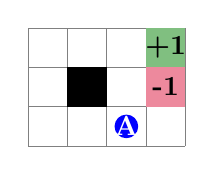
\begin{tikzpicture}[scale=0.5]
                % Grid
                \draw[step=1cm,gray,very thin] (0,0) grid (4,3);
                
                % Walls
                \fill[black] (1,1) rectangle (2,2);
                
                % Goal
                \fill[green!50] (3,2) rectangle (4,3);
                \node at (3.5,2.5) {\textbf{+1}};
                
                % Penalty
                \fill[red!50] (3,1) rectangle (4,2);
                \node at (3.5,1.5) {\textbf{-1}};
                
                % Agent position
                \fill[blue] (2.5,0.5) circle (0.3);
                \node at (2.5,0.5) {\color{white}\textbf{A}};
            \end{tikzpicture}

        \end{column}
        
        \begin{column}{0.55\textwidth}
            
            
            
            $$\rho \gets \text{uniform random number in } [0,1] = 0.65 $$
            
            \textbf{Action selection:} \\
            \eIf{$\rho = 0.65 < \epsilon = 0.1$}{
                Choose random action $a \in A$ $\rightarrow$
            }{
                $a \gets \argmax_{a \in A} Q((2,0), a) = \argmax_{a \in A} \{0, -0.004, 0, 0\}$
            }

             Tie break (between Up, Left, and Right): agent randomly selects Up action
        \end{column}
    \end{columns}
\end{frame}

\begin{frame}{Q-Value Update Example - Step 6 (continued)}

    \begin{columns}
        \begin{column}{0.5\textwidth}
            \textbf{Q-Table Before Update}
            \small
            \begin{table}[h]
                \centering
                \begin{tabular}{|c|c|c|c|c|}
                    \hline
                    \textbf{State} & \textbf{Up} & \textbf{Down} & \textbf{Left} & \textbf{Right} \\
                    \hline
                    (0,0) & 0.000 & 0.000 & 0.000 & \textcolor{red}{-0.004} \\
                    (1,0) & \textcolor{red}{-0.004} & 0.000 & 0.000 & \textcolor{red}{-0.004} \\
                    (2,0) & 0.000 & \textcolor{red}{-0.004} & 0.000 & 0.000 \\
                    (3,0) & 0.000 & 0.000 & \textcolor{red}{-0.004} & 0.000 \\
                    \dots & \dots & \dots & \dots & \dots \\
                    \hline
                \end{tabular}
            \end{table}
            
            \textbf{Q-Table After Update}
            \small
            \begin{table}[h]
                \centering
                \begin{tabular}{|c|c|c|c|c|}
                    \hline
                    \textbf{State} & \textbf{Up} & \textbf{Down} & \textbf{Left} & \textbf{Right} \\
                    \hline
                    (0,0) & 0.000 & 0.000 & 0.000 & \textcolor{red}{-0.004} \\
                    (1,0) & \textcolor{red}{-0.004} & 0.000 & 0.000 & \textcolor{red}{-0.004} \\
                    (2,0) & \textcolor{blue}{-0.004} & \textcolor{red}{-0.004} & 0.000 & 0.000 \\
                    (3,0) & 0.000 & 0.000 & \textcolor{red}{-0.004} & 0.000 \\
                    \dots & \dots & \dots & \dots & \dots \\
                    \hline
                \end{tabular}
            \end{table}
        \end{column}
        
        \begin{column}{0.5\textwidth}
            
            \begin{align}
                s &= (2,0), \quad a = \text{Up} \\
                s' &= (2,1), \quad r = -0.04 \\
                \max_{a'}Q(s',a') &= 0 \\
                Q((2,0),\text{Up}) &= 0 + 0.1[-0.04 + 0.9 \cdot 0 - 0] \\
                &= \textcolor{blue}{-0.004}
            \end{align}
            
            \vspace{0.5cm}
            \textbf{Current State:} Agent goes to $(2,1)$
        \end{column}
    \end{columns}
\end{frame}



\begin{frame}{Q-Value Update Example - Step 7}
    
    \begin{columns}
        \begin{column}{0.45\textwidth}
            \textbf{Q-Table}
            \small
            \begin{table}[h]
                \centering
                \begin{tabular}{|c|c|c|c|c|}
                    \hline
                    \textbf{State} & \textbf{Up} & \textbf{Down} & \textbf{Left} & \textbf{Right} \\
                    \hline
                    (0,0) & 0.000 & 0.000 & 0.000 & \textcolor{red}{-0.004} \\
                    (1,0) & \textcolor{red}{-0.004} & 0.000 & 0.000 & \textcolor{red}{-0.004} \\
                    (2,0) & \textcolor{red}{-0.004} & \textcolor{red}{-0.004} & 0.000 & 0.000 \\
                    (3,0) & 0.000 & 0.000 & \textcolor{red}{-0.004} & 0.000 \\
                    (2,1) & 0.000 & 0.000 & 0.000 & 0.000 \\
                    (2,2) & 0.000 & 0.000 & 0.000 & 0.000 \\
                    (3,1) & 0.000 & 0.000 & 0.000 & 0.000 \\
                    \dots & \dots & \dots & \dots & \dots \\
                    \hline
                \end{tabular}
            \end{table}
            
            \textbf{Current State:} Agent at (2,1)

            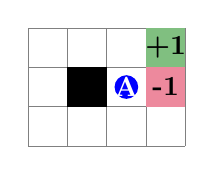
\begin{tikzpicture}[scale=0.5]
                % Grid
                \draw[step=1cm,gray,very thin] (0,0) grid (4,3);
                
                % Walls
                \fill[black] (1,1) rectangle (2,2);
                
                % Goal
                \fill[green!50] (3,2) rectangle (4,3);
                \node at (3.5,2.5) {\textbf{+1}};
                
                % Penalty
                \fill[red!50] (3,1) rectangle (4,2);
                \node at (3.5,1.5) {\textbf{-1}};
                
                % Agent position
                \fill[blue] (2.5,1.5) circle (0.3);
                \node at (2.5,1.5) {\color{white}\textbf{A}};
            \end{tikzpicture}

        \end{column}
        
        \begin{column}{0.55\textwidth}
            
            
            
            $$\rho \gets \text{uniform random number in } [0,1] = 0.82 $$
            
            \textbf{Action selection:} \\
            \eIf{$\rho = 0.82 < \epsilon = 0.1$}{
                Choose random action $a \in A$ $\rightarrow$
            }{
                $a \gets \argmax_{a \in A} Q((2,1), a) = \argmax_{a \in A} \{0, 0, 0, 0\}$
            }

             Tie break: agent randomly selects Up action
        \end{column}
    \end{columns}
\end{frame}

\begin{frame}{Q-Value Update Example - Step 7 (continued)}

    \begin{columns}
        \begin{column}{0.5\textwidth}
            \textbf{Q-Table Before Update}
            \small
            \begin{table}[h]
                \centering
                \begin{tabular}{|c|c|c|c|c|}
                    \hline
                    \textbf{State} & \textbf{Up} & \textbf{Down} & \textbf{Left} & \textbf{Right} \\
                    \hline
                    (0,0) & 0.000 & 0.000 & 0.000 & \textcolor{red}{-0.004} \\
                    (1,0) & \textcolor{red}{-0.004} & 0.000 & 0.000 & \textcolor{red}{-0.004} \\
                    (2,0) & \textcolor{red}{-0.004} & \textcolor{red}{-0.004} & 0.000 & 0.000 \\
                    (3,0) & 0.000 & 0.000 & \textcolor{red}{-0.004} & 0.000 \\
                    (2,1) & 0.000 & 0.000 & 0.000 & 0.000 \\
                    (2,2) & 0.000 & 0.000 & 0.000 & 0.000 \\
                    \dots & \dots & \dots & \dots & \dots \\
                    \hline
                \end{tabular}
            \end{table}
            
           
        \end{column}
        
        \begin{column}{0.5\textwidth}
            
             \textbf{Q-Table After Update}
            \small
            \begin{table}[h]
                \centering
                \begin{tabular}{|c|c|c|c|c|}
                    \hline
                    \textbf{State} & \textbf{Up} & \textbf{Down} & \textbf{Left} & \textbf{Right} \\
                    \hline
                    (0,0) & 0.000 & 0.000 & 0.000 & \textcolor{red}{-0.004} \\
                    (1,0) & \textcolor{red}{-0.004} & 0.000 & 0.000 & \textcolor{red}{-0.004} \\
                    (2,0) & \textcolor{red}{-0.004} & \textcolor{red}{-0.004} & 0.000 & 0.000 \\
                    (3,0) & 0.000 & 0.000 & \textcolor{red}{-0.004} & 0.000 \\
                    (2,1) & \textcolor{blue}{-0.004} & 0.000 & 0.000 & 0.000 \\
                    (2,2) & 0.000 & 0.000 & 0.000 & 0.000 \\
                    \dots & \dots & \dots & \dots & \dots \\
                    \hline
                \end{tabular}
            \end{table}

            
        \end{column}
    \end{columns}

    \vspace{-5mm}
    \begin{align}
                s &= (2,1), \quad a = \text{Up} \\
                s' &= (2,2), \quad r = -0.04 \\
                & \max_{a'}Q(s',a') = 0 \\
                Q((2,1),\text{Up}) &= 0 + 0.1[-0.04 + 0.9 \cdot 0 - 0] = \textcolor{blue}{-0.004}
            \end{align}
            
            
            \textbf{Current State:} Agent goes to $(2,2)$
\end{frame}




\begin{frame}{Q-Value Update Example - Step 8}
    
    \begin{columns}
        \begin{column}{0.45\textwidth}
            \textbf{Q-Table}
            \small
            \begin{table}[h]
                \centering
                \begin{tabular}{|c|c|c|c|c|}
                    \hline
                    \textbf{State} & \textbf{Up} & \textbf{Down} & \textbf{Left} & \textbf{Right} \\
                    \hline
                    (0,0) & 0.000 & 0.000 & 0.000 & \textcolor{red}{-0.004} \\
                    (1,0) & \textcolor{red}{-0.004} & 0.000 & 0.000 & 0.000 \\
                    (2,0) & \textcolor{red}{-0.004} & \textcolor{red}{-0.004} & 0.000 & 0.000 \\
                    (3,0) & 0.000 & 0.000 & \textcolor{red}{-0.004} & 0.000 \\
                    (2,1) & \textcolor{red}{-0.004} & 0.000 & 0.000 & 0.000 \\
                    (2,2) & 0.000 & 0.000 & 0.000 & 0.000 \\
                    \dots & \dots & \dots & \dots & \dots \\
                    \hline
                \end{tabular}
            \end{table}
            
            \textbf{Current State:} Agent at (2,2)

            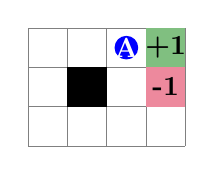
\begin{tikzpicture}[scale=0.5]
                % Grid
                \draw[step=1cm,gray,very thin] (0,0) grid (4,3);
                
                % Walls
                \fill[black] (1,1) rectangle (2,2);
                
                % Goal
                \fill[green!50] (3,2) rectangle (4,3);
                \node at (3.5,2.5) {\textbf{+1}};
                
                % Penalty
                \fill[red!50] (3,1) rectangle (4,2);
                \node at (3.5,1.5) {\textbf{-1}};
                
                % Agent position
                \fill[blue] (2.5,2.5) circle (0.3);
                \node at (2.5,2.5) {\color{white}\textbf{A}};
            \end{tikzpicture}


        \end{column}
        
        \begin{column}{0.55\textwidth}
            
            
            
            $$\rho \gets \text{uniform random number in } [0,1] = 0.22 $$
            
            \textbf{Action selection:} \\
            \eIf{$\rho = 0.22 < \epsilon = 0.1$}{
                Choose random action $a \in A$ $\rightarrow$
            }{
                $a \gets \argmax_{a \in A} Q((2,2), a) = \argmax_{a \in A} \{0, 0, 0, 0\}$
            }

             Tie break: agent randomly selects Right action
        \end{column}
    \end{columns}
\end{frame}

\begin{frame}{Q-Value Update Example - Step 8 (continued)}

    \begin{columns}
        
        \begin{column}{0.5\textwidth}
            \textbf{Q-Table Before Update}
            \small
            \begin{table}[h]
                \centering
                \begin{tabular}{|c|c|c|c|c|}
                    \hline
                    \textbf{State} & \textbf{Up} & \textbf{Down} & \textbf{Left} & \textbf{Right} \\
                    \hline
                    (0,0) & 0.000 & 0.000 & 0.000 & \textcolor{red}{-0.004} \\
                    (1,0) & \textcolor{red}{-0.004} & 0.000 & 0.000 & 0.000 \\
                    (2,0) & \textcolor{red}{-0.004} & \textcolor{red}{-0.004} & 0.000 & 0.000 \\
                    (3,0) & 0.000 & 0.000 & \textcolor{red}{-0.004} & 0.000 \\
                    (2,1) & \textcolor{red}{-0.004} & 0.000 & 0.000 & 0.000 \\
                    (2,2) & 0.000 & 0.000 & 0.000 & 0.000 \\
                    \dots & \dots & \dots & \dots & \dots \\
                    \hline
                \end{tabular}
            \end{table}
            
            \vspace{0.5cm}
            
            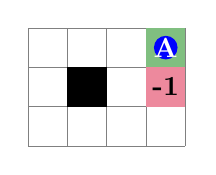
\begin{tikzpicture}[scale=0.5]
                % Grid
                \draw[step=1cm,gray,very thin] (0,0) grid (4,3);
                
                % Walls
                \fill[black] (1,1) rectangle (2,2);
                
                % Goal
                \fill[green!50] (3,2) rectangle (4,3);
                % \node at (3.5,2.5) {\textbf{+1}};
                
                % Penalty
                \fill[red!50] (3,1) rectangle (4,2);
                \node at (3.5,1.5) {\textbf{-1}};
                
                % Agent position
                \fill[blue] (3.5,2.5) circle (0.3);
                \node at (3.5,2.5) {\color{white}\textbf{A}};
            \end{tikzpicture}

            
        \end{column}
        
        \begin{column}{0.5\textwidth}

            \textbf{Q-Table After Update}
            \small
            \begin{table}[h]
                \centering
                \begin{tabular}{|c|c|c|c|c|}
                    \hline
                    \textbf{State} & \textbf{Up} & \textbf{Down} & \textbf{Left} & \textbf{Right} \\
                    \hline
                    (0,0) & 0.000 & 0.000 & 0.000 & \textcolor{red}{-0.004} \\
                    (1,0) & \textcolor{red}{-0.004} & 0.000 & 0.000 & \textcolor{red}{-0.004} \\
                    (2,0) & \textcolor{red}{-0.004} & \textcolor{red}{-0.004} & 0.000 & 0.000 \\
                    (3,0) & 0.000 & 0.000 & \textcolor{red}{-0.004} & 0.000 \\
                    (2,1) & \textcolor{red}{-0.004} & 0.000 & 0.000 & 0.000 \\
                    (2,2) & 0.000 & 0.000 & 0.000 & \textcolor{blue}{0.1} \\
                    \dots & \dots & \dots & \dots & \dots \\
                    \hline
                \end{tabular}
            \end{table}

            \vspace{-0.82cm}

                \begin{align}
                s &= (2,2), \quad a = \text{Right} \\
                s' &= (3,2), \quad r = +1 \\
                & \max_{a'}Q(s',a') = 0 \\
                Q((2,2),\text{Right}) &= 0 + 0.1[1 + 0.9 \cdot 0 - 0] = \textcolor{blue}{0.1}
            \end{align}
            
            
            

        \end{column}
    \end{columns}

    \textbf{Current State:} Agent goes to $(3,2)$

\end{frame}




%%%%%%%%%%%%%%%%%%%%%%%%%





\begin{frame}{Q-Value Update Example - Final State}
    
    \begin{columns}
        \begin{column}{0.6\textwidth}
            \textbf{Final Q-Table}
            \small
            \begin{table}[h]
                \centering
                \begin{tabular}{|c|c|c|c|c|}
                    \hline
                    \textbf{State} & \textbf{Up} & \textbf{Down} & \textbf{Left} & \textbf{Right} \\
                    \hline
                    (0,0) & 0.000 & 0.000 & 0.000 & \textcolor{red}{-0.004} \\
                    (1,0) & \textcolor{red}{-0.004} & 0.000 & 0.000 & \textcolor{red}{-0.004} \\
                    (2,0) & \textcolor{red}{-0.004} & \textcolor{red}{-0.004} & 0.000 & 0.000 \\
                    (3,0) & 0.000 & 0.000 & \textcolor{red}{-0.004} & 0.000 \\
                    (2,1) & \textcolor{red}{-0.004} & 0.000 & 0.000 & 0.000 \\
                    (2,2) & 0.000 & 0.000 & 0.000 & \textcolor{blue}{0.1} \\
                    (3,1) & 0.000 & 0.000 & 0.000 & 0.000 \\
                    (3,2) & 0.000 & 0.000 & 0.000 & 0.000 \\
                    \dots & \dots & \dots & \dots & \dots \\
                    \hline
                \end{tabular}
            \end{table}
        \end{column}
        
        \begin{column}{0.4\textwidth}
            \textbf{Key Insights:}
            \begin{itemize}
                \item Only visited state-action pairs get updated
                \item \textbf{Episode:} From start until agent reaches terminal state, e.g., reward $+1$ or $-1$.
                \item \textbf{Step:} Each action taken by the agent within an episode.
                \item Learning is incremental and experience-based
            \end{itemize}
            
        \end{column}
    \end{columns}
\end{frame}

\begin{frame}{Training Structure: Runs, Episodes, and Steps}
    \begin{columns}
        \begin{column}{0.55\textwidth}
            \begin{algorithm}[H]
                \caption{Q-Learning Training Structure}
                \SetAlgoLined
                \footnotesize
                \For{run = 1 to num\_runs}{
                    Initialize $Q(s,a) = 0 \ \forall \ s \in S, a \in A$\;
                    \For{episode = 1 to max\_episodes}{
                        Initialize state $s = s_{start}$\;
                        $step = 0$\;
                        \While{$s$ not terminal AND $step < max\_steps$}{
                            Choose action $a$ using $\epsilon$-greedy\;
                            Execute action $a$, observe $s'$ and $r$\;
                            Update: $Q(s,a) \leftarrow Q(s,a) + \alpha[r + \gamma \max_{a'}Q(s',a') - Q(s,a)]$\;
                            $s \leftarrow s'$, $step \leftarrow step + 1$\;
                        }
                        \If{episode \% test\_interval == 0}{
                            Evaluate current policy\;
                        }
                    }
                    % Save Q-table and performance metrics\;
                }
            \end{algorithm}
        \end{column}
        \begin{column}{0.4\textwidth}
            \textbf{Hierarchical Structure:}
            \begin{itemize}
                \item \textbf{Run (iteration):} Complete training process with independent initialization
                \item \textbf{Episode:} Single game from start to terminal state
                \item \textbf{Step:} Individual action taken within an episode
            \end{itemize}
            
            % \vspace{0.5cm}
            \textbf{Our Configuration:}
            \begin{itemize}
                \item \textbf{Runs:} 5 independent runs
                \item \textbf{Episodes:} 5000 per run
                \item \textbf{Steps:} Max 80 per episode
                \item \textbf{Testing:} Every 20 episodes
            \end{itemize}
        \end{column}
    \end{columns}
\end{frame}

\section{Results and Analysis}

% \begin{frame}{Optimal Policy Visualization}
%     \begin{center}
%         \textbf{Learned Optimal Policy:}
%         \vspace{0.5cm}
        
%         \begin{tabular}{c|cccc}
%             & \textbf{x=1} & \textbf{x=2} & \textbf{x=3} & \textbf{x=4} \\
%             \hline
%             \textbf{y=3} & $\rightarrow$ & $\rightarrow$ & $\rightarrow$ & \textcolor{green}{\textbf{+1}} \\
%             \textbf{y=2} & $\uparrow$ & \textbf{XX} & $\uparrow$ & \textcolor{red}{\textbf{-200}} \\
%             \textbf{y=1} & \textcolor{blue}{\textbf{S}}$\uparrow$ & $\leftarrow$ & $\uparrow$ & $\leftarrow$ \\
%         \end{tabular}
%     \end{center}
    
%     \vspace{0.5cm}
%     \textbf{Optimal Path:} (0,0) $\rightarrow$ (0,1) $\rightarrow$ (0,2) $\rightarrow$ (1,2) $\rightarrow$ (2,2) $\rightarrow$ (3,2)
    
%     \textbf{Expected Total Reward:} 0.84 (accounting for step costs and slip probability)
% \end{frame}

% \begin{frame}{Animated GIF Example}
%     \centering
%     \animategraphics[loop,autoplay,width=0.8\linewidth]{10}{./Results/frame-}{0}{5}
% \end{frame}





\begin{frame}{Training Animation}
    \begin{center}
        \textbf{Agent Following Optimal Policy - Training}
        \vspace{0.5cm}
        
        % Training animation GIF (for presentation software that supports it)
        % \animategraphics[loop,controls,width=0.7\textwidth]{1.2}{./Results/optimal_policy_animation_train_iter_}{1}{5}
        
        % Static visualization for LaTeX compilation
            \begin{figure}[h]
                \centering
                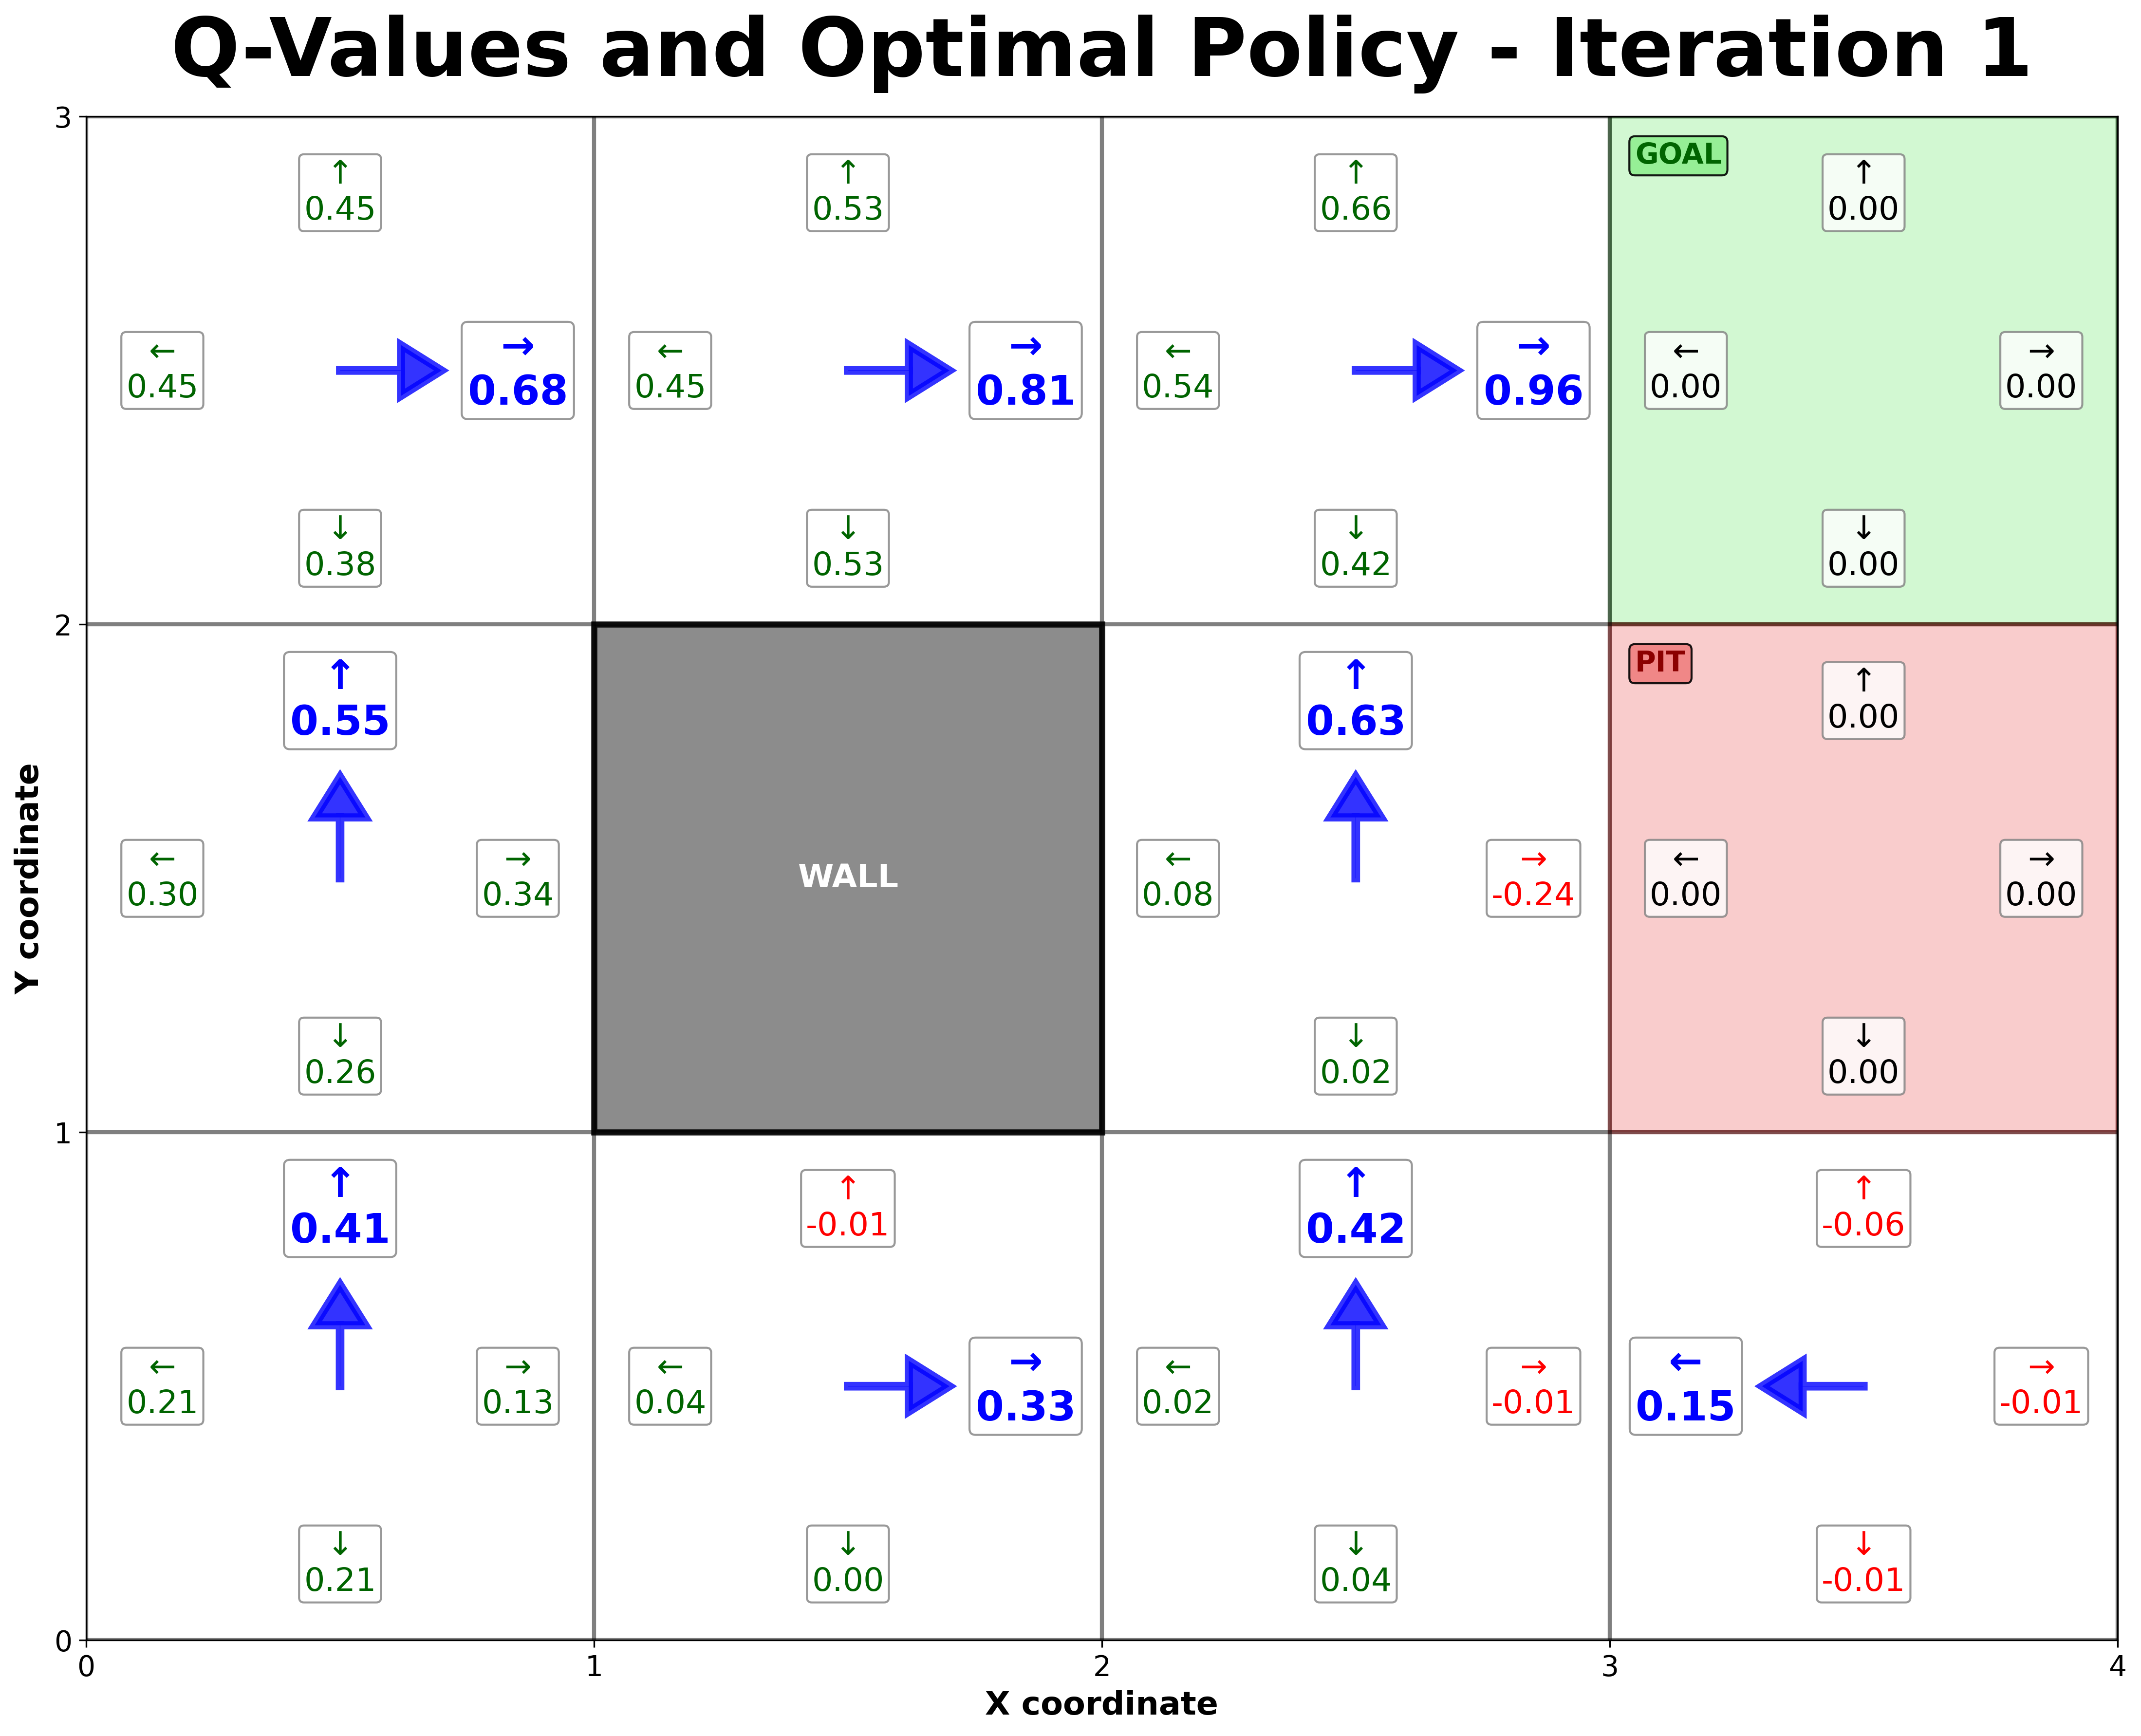
\includegraphics[width=0.45\textwidth]{./Results/optimal_policy_reward_minus_1.png}
                \caption{Optimal policy for the case with penalty of $-1$.}
            \end{figure}
        

        
        \vspace{0.3cm}
        \small{
       Optimal policy for the case with penalty of $-1$.}
    \end{center}
\end{frame}



\begin{frame}{Training Animation}
    \begin{center}
        \textbf{Agent Following Optimal Policy - Training}
        \vspace{0.5cm}
        
        % Training animation GIF (for presentation software that supports it)
        % \animategraphics[loop,controls,width=0.7\textwidth]{1.2}{./Results/optimal_policy_animation_train_iter_}{1}{5}
        
        % Static visualization for LaTeX compilation
                    \begin{figure}[h]
                \centering
                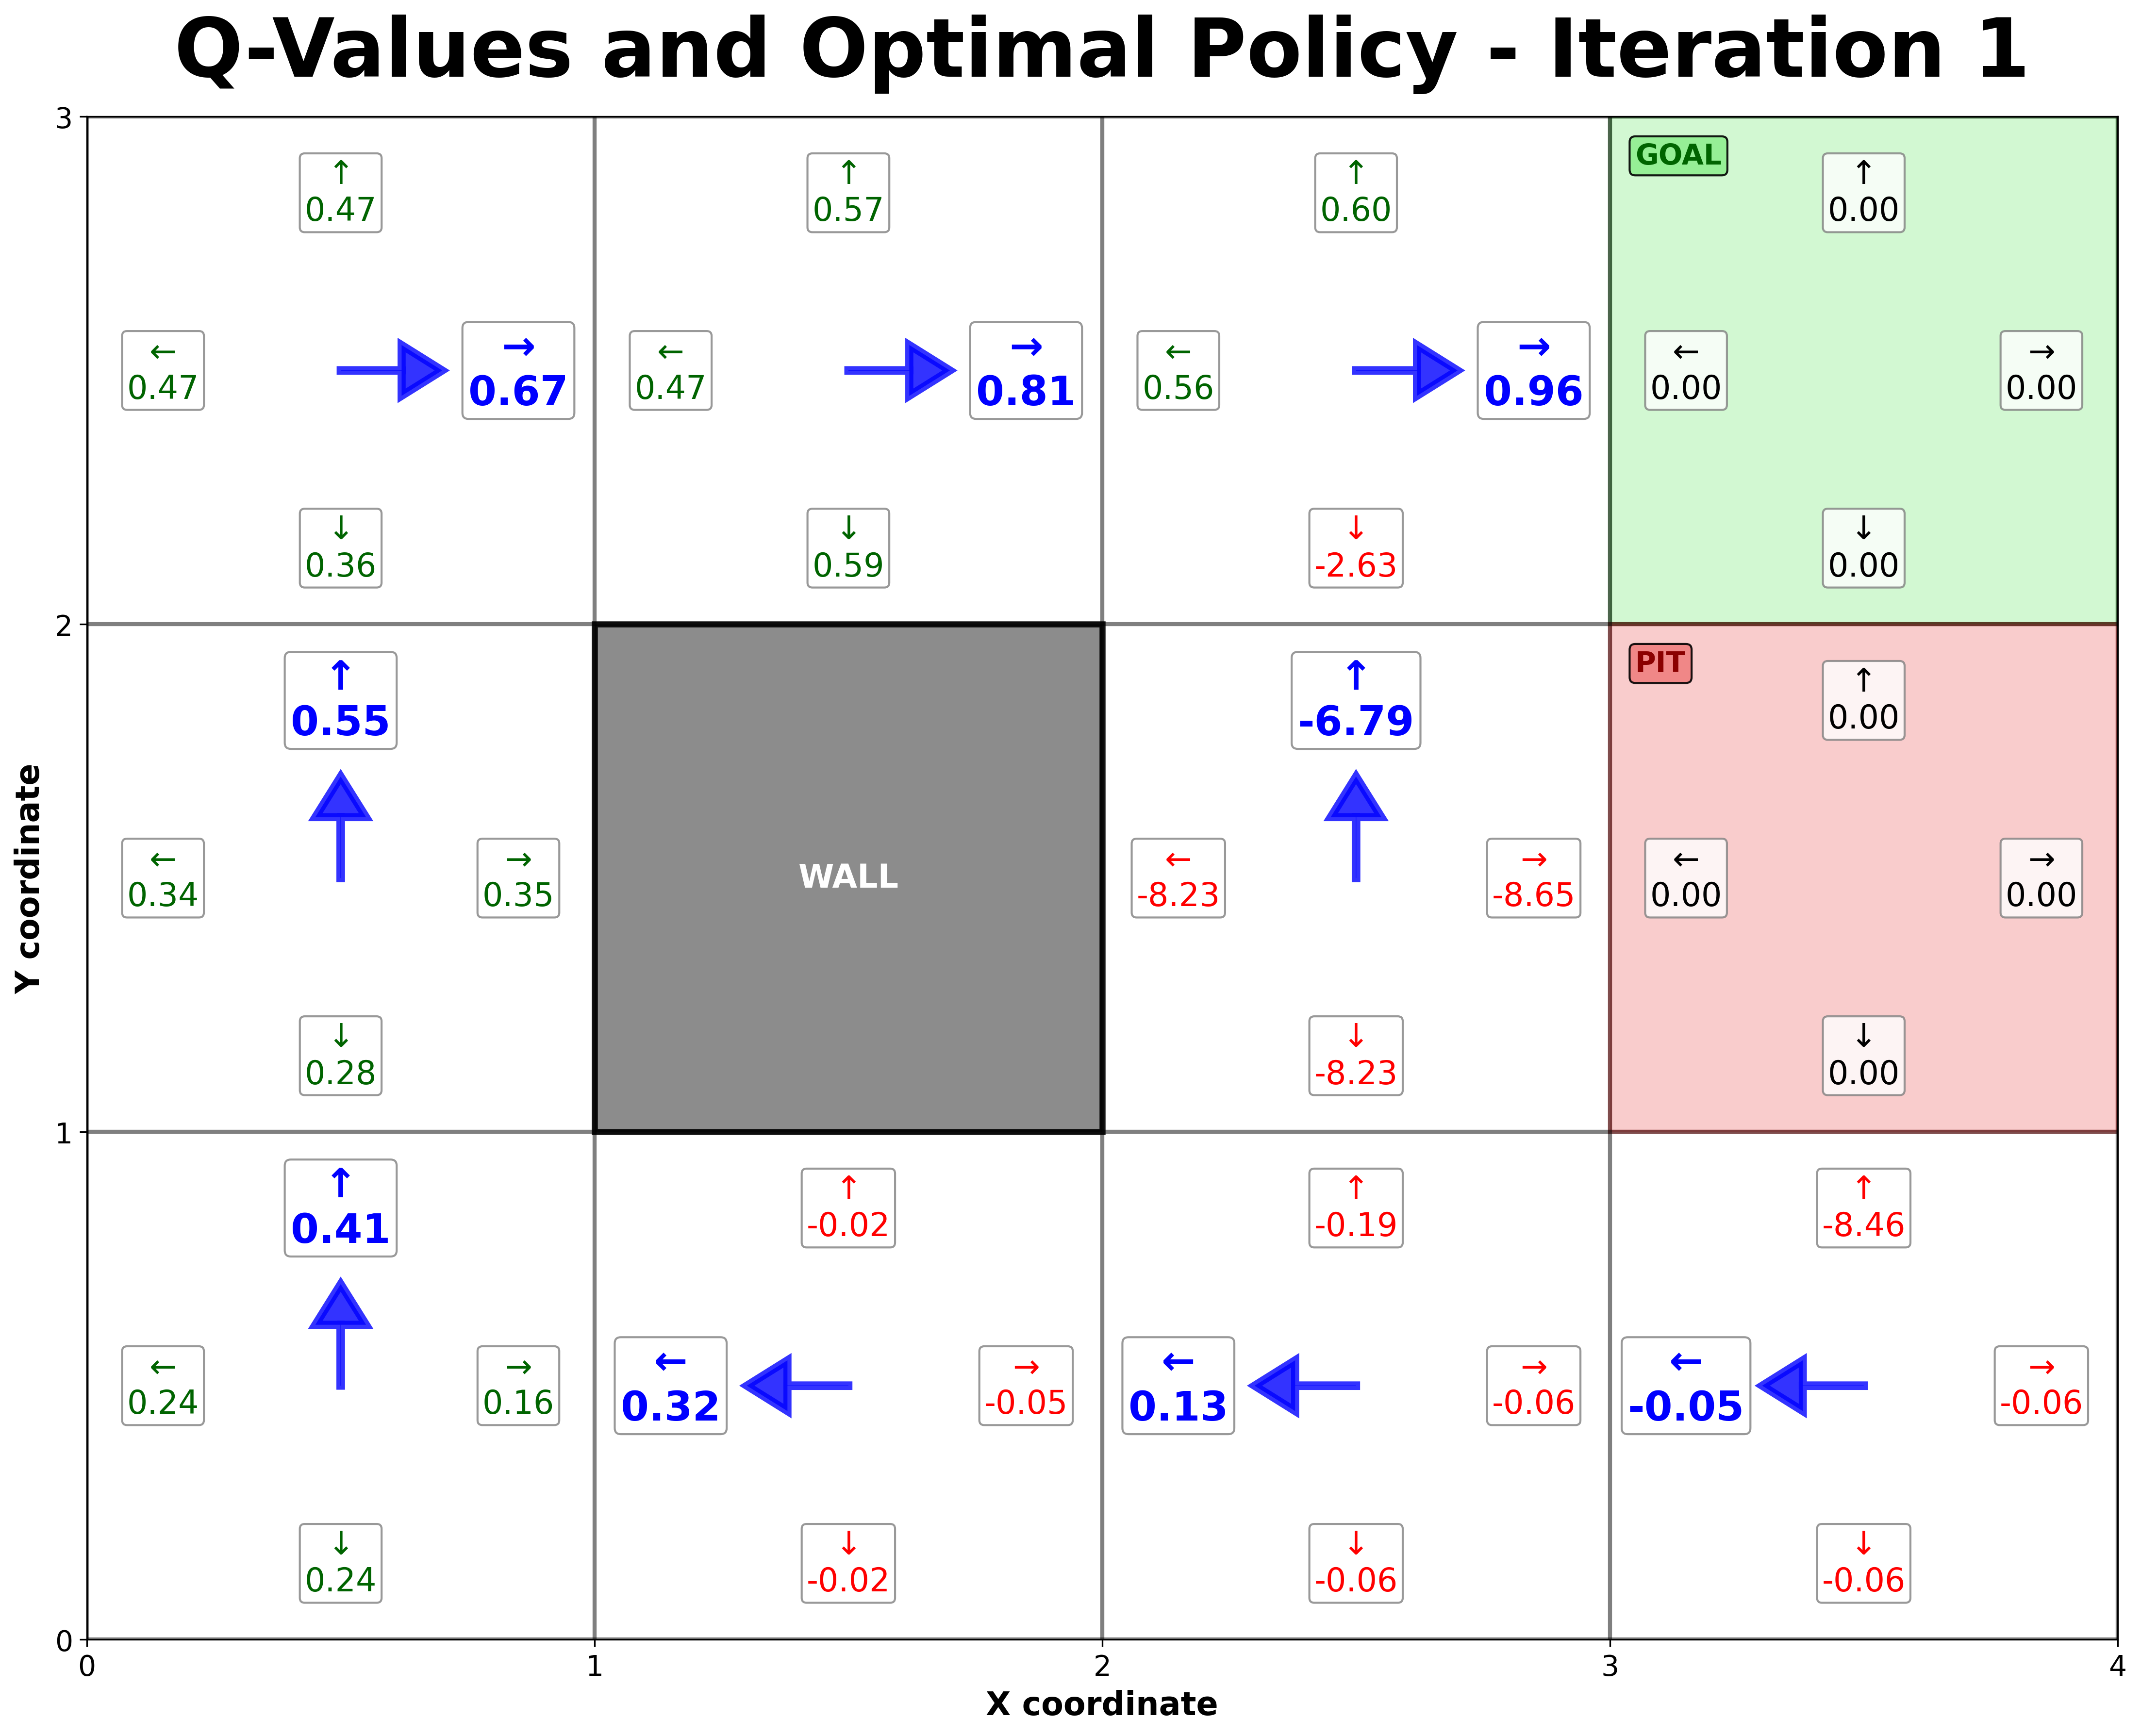
\includegraphics[width=0.45\textwidth]{./Results/optimal_policy_reward_minus_100.png}
                \caption{Optimal policy for the case with penalty of $-100$.}
            \end{figure}
        
        
        \vspace{0.3cm}
        \small{
       Optimal policy for the case with penalty of $-100$.}
    \end{center}
\end{frame}

\begin{frame}{Training Performance}
    \begin{columns}
        \begin{column}{0.6\textwidth}
            \begin{figure}[h]
                \centering
                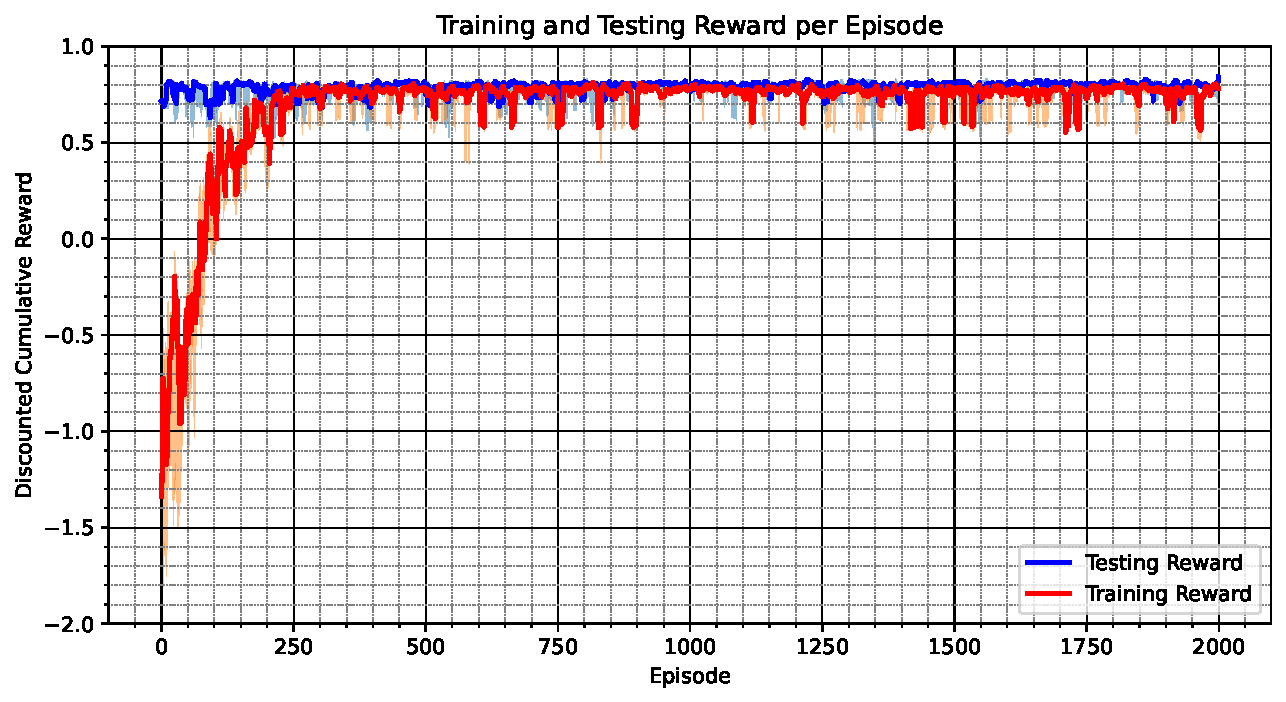
\includegraphics[width=\textwidth]{./Results/agent_reward.pdf}
                \caption{Training performance over 5000 episodes. Each curve represents the average reward over 5 independent runs. Shaded areas indicate percentile data.}
            \end{figure}
        \end{column}
        \begin{column}{0.4\textwidth}
            \textbf{Training Configuration:}
            \begin{itemize}
                \item 5 independent runs per parameter setting
                \item 5000 training episodes per run
                \item Testing every 100 episodes
                \item Performance measured by average testing reward
            \end{itemize}
        \end{column}
    \end{columns}
\end{frame}

\section{Parameter Study}

\begin{frame}{Parameter Study Setup}
    \textbf{Hyperparameter Ranges:}
    \begin{columns}
        \begin{column}{0.33\textwidth}
            \textbf{Learning Rate ($\alpha$):}
            \begin{itemize}
                \item 0.01
                \item 0.1
                \item 0.5
                \item 0.9
            \end{itemize}
        \end{column}
        \begin{column}{0.33\textwidth}
            \textbf{Discount Factor ($\gamma$):}
            \begin{itemize}
                \item 0.1
                \item 0.3
                \item 0.9
                \item 0.95
            \end{itemize}
        \end{column}
        \begin{column}{0.33\textwidth}
            \textbf{Exploration Rate ($\epsilon$):}
            \begin{itemize}
                \item 0.01
                \item 0.1
                \item 0.3
                \item 0.5
            \end{itemize}
        \end{column}
    \end{columns}
    
    \vspace{0.5cm}
    \textbf{Study Configuration:}
    \begin{itemize}
        \item 5000 training episodes per run
        \item Testing every 100 episodes
        \item Performance measured by average testing reward
    \end{itemize}
\end{frame}

\begin{frame}{Parameter Study Results - Learning Rate}
    \begin{center}
        
        % Parameter study plots (update with actual filenames when generated)
        \begin{figure}[h]
            \centering
            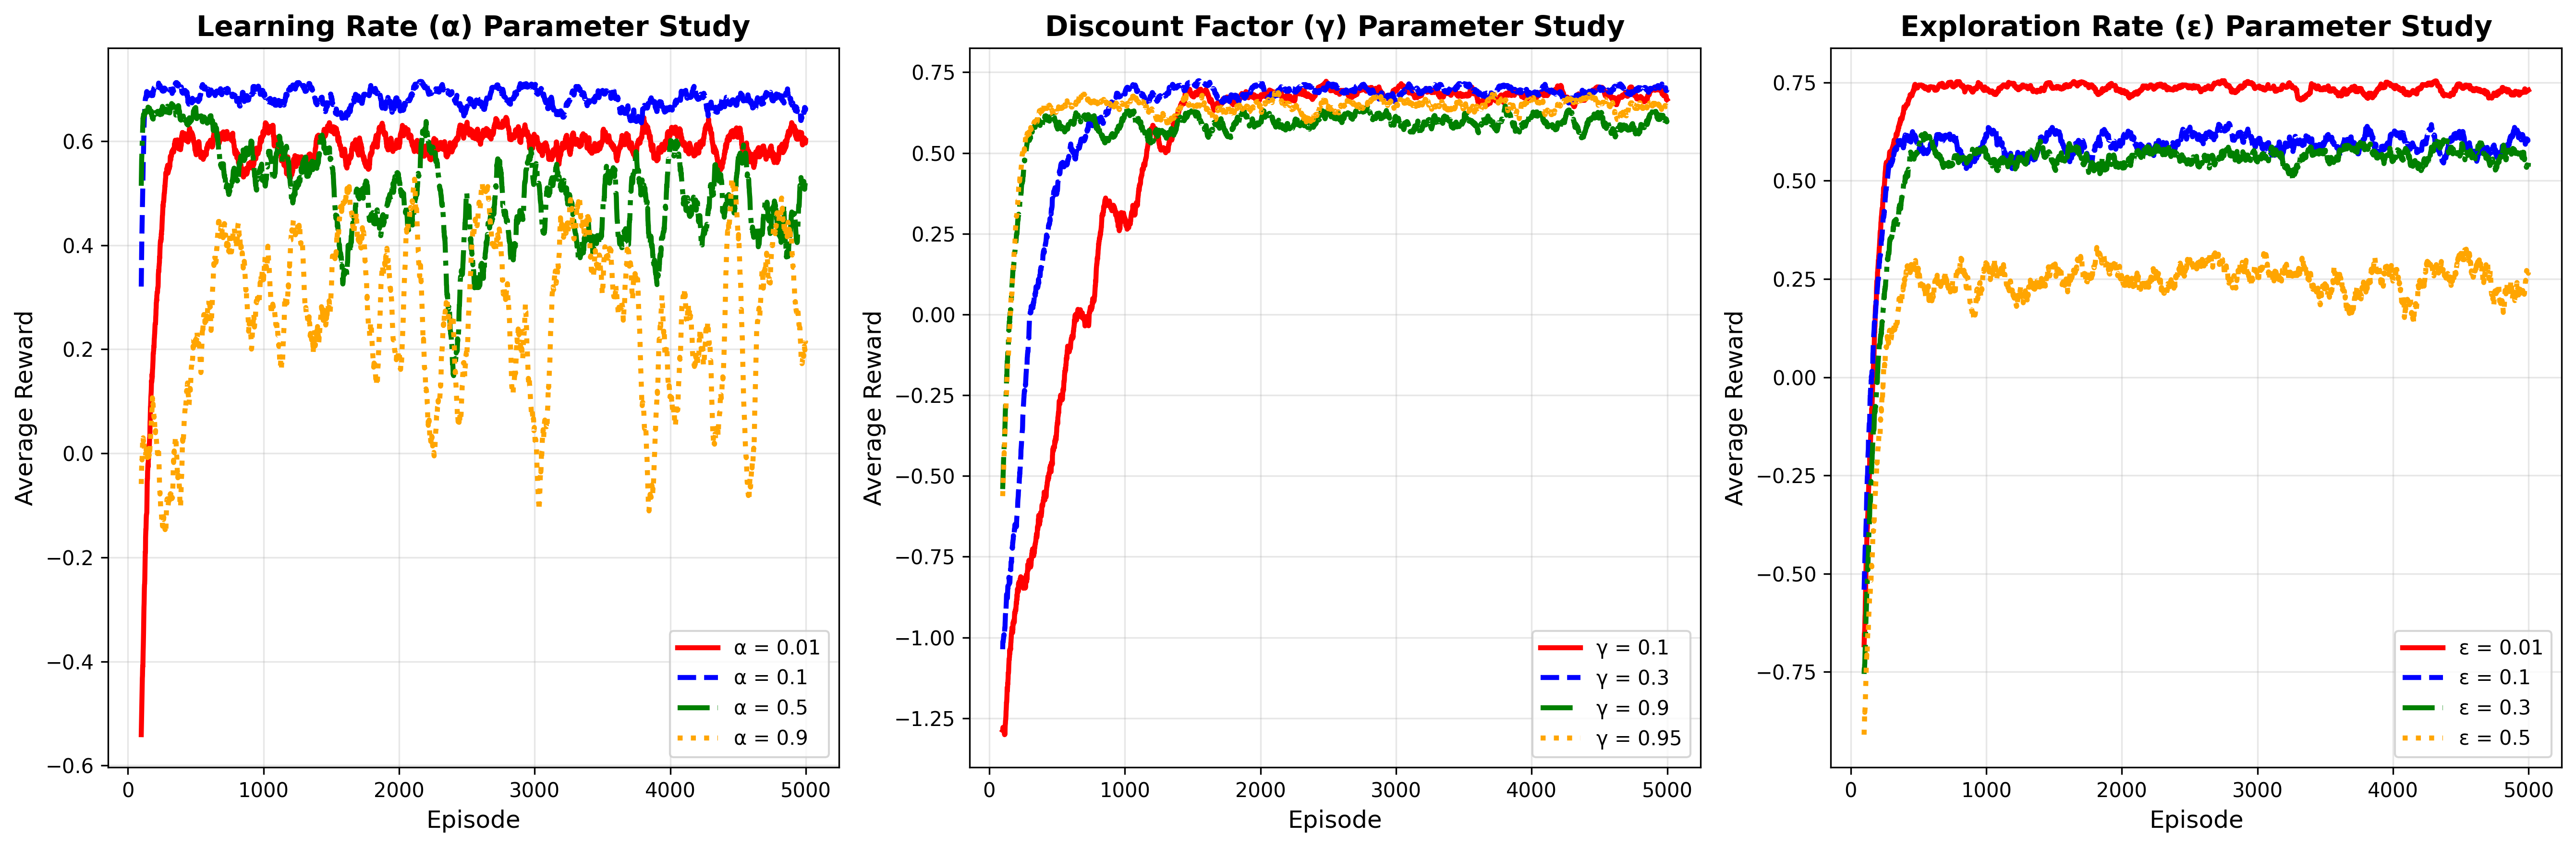
\includegraphics[width=0.8\textwidth]{./Results/parameter_study_curves.png}
            \caption{Training performance for different learning rates, discount factors, and exploration rates. Each curve represents the average reward over 5 independent runs.}
        \end{figure}
        
        \textbf{Key Findings:}
        \begin{itemize}
            \item Higher learning rates cause instability
            \item Higher discount factors better capture long-term rewards
            \item High exploration rates result in lower final performance
        \end{itemize}
    \end{center}
\end{frame}

% \begin{frame}{Parameter Study Results - Discount Factor}
%     \begin{center}
%         \textbf{Effect of Discount Factor ($\gamma$)}
%         \vspace{0.3cm}
        
%         \begin{figure}[h]
%             \centering
%             \includegraphics[width=0.8\textwidth]{./Results/gamma_parameter_study_curves.png}
%         \end{figure}
        
%         \textbf{Key Findings:}
%         \begin{itemize}
%             \item Higher discount factors (0.9, 0.95) achieve better long-term performance
%             \item Lower discount factors (0.1, 0.3) focus on immediate rewards
%             \item Optimal value: $\gamma = 0.9$ balances future and immediate rewards
%         \end{itemize}
%     \end{center}
% \end{frame}

% \begin{frame}{Parameter Study Results - Exploration Rate}
%     \begin{center}
%         \textbf{Effect of Exploration Rate ($\epsilon$)}
%         \vspace{0.3cm}
        
%         \begin{figure}[h]
%             \centering
%             \includegraphics[width=0.8\textwidth]{./Results/epsilon_parameter_study_curves.png}
%         \end{figure}
        
%         \textbf{Key Findings:}
%         \begin{itemize}
%             \item Very low exploration (0.01) may get stuck in suboptimal policies
%             \item Very high exploration (0.5) slows down convergence
%             \item Optimal range: $\epsilon \in [0.1, 0.3]$ for this environment
%         \end{itemize}
%     \end{center}
% \end{frame}

% \begin{frame}{Final Performance Comparison}
%     \begin{center}
        
%         \begin{figure}[h]
%             \centering
%             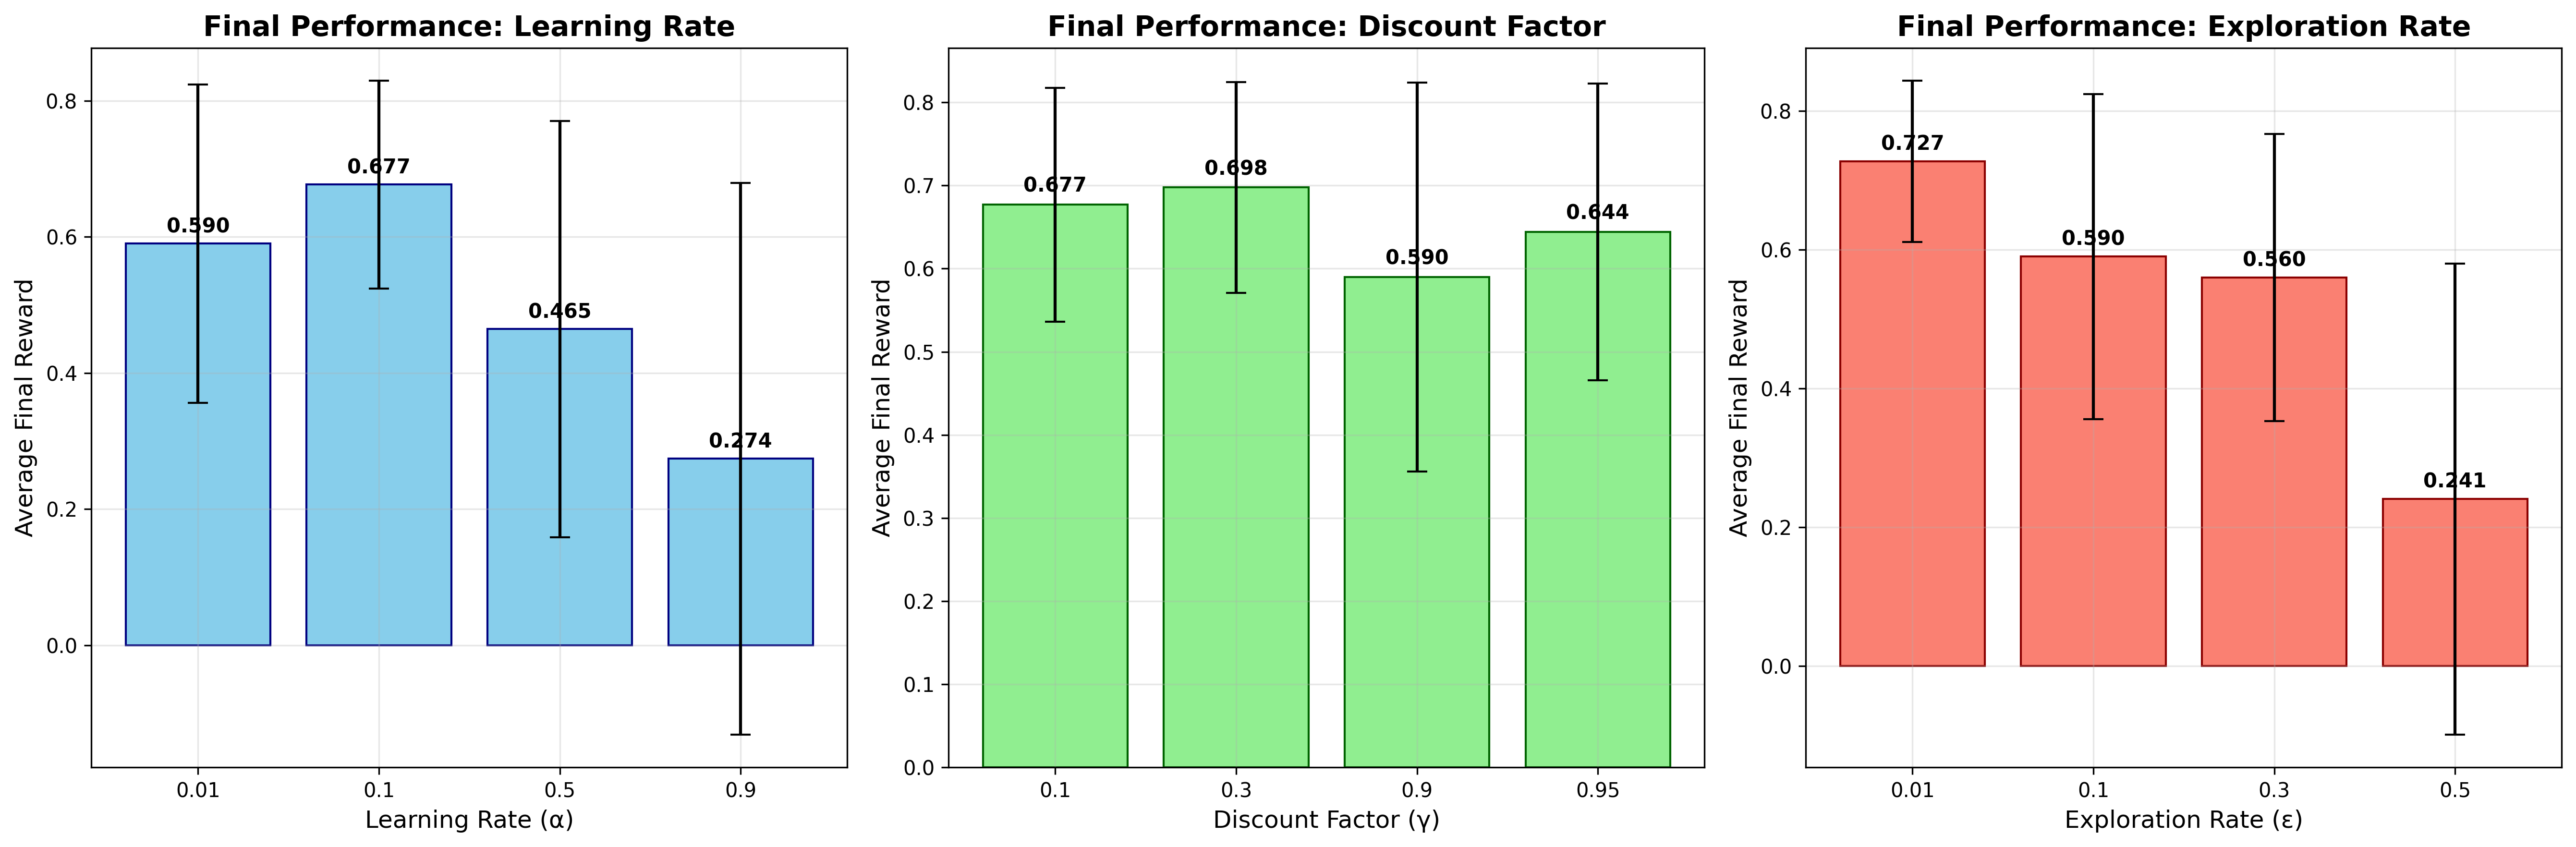
\includegraphics[width=0.9\textwidth]{./Results/parameter_study_final_performance.png}
%             \caption{Increase in learning rate leads to less stable performance.}
%         \end{figure}
        
%         % \begin{table}[h]
%         %     \centering
%         %     \begin{tabular}{|c|c|c|c|}
%         %         \hline
%         %         \textbf{Parameter} & \textbf{Best Value} & \textbf{Final Reward} & \textbf{Convergence Episodes} \\
%         %         \hline
%         %         Learning Rate & 0.1 & 0.85 & 2000 \\
%         %         Discount Factor & 0.9 & 0.84 & 1800 \\
%         %         Exploration Rate & 0.1 & 0.84 & 1900 \\
%         %         \hline
%         %     \end{tabular}
%         %     \caption{Best performing hyperparameter values and their corresponding final average rewards.}
%         % \end{table}
%     \end{center}
% \end{frame}



\section{Conclusions}

\begin{frame}{Key Findings}
    \textbf{Algorithm Performance:}
    \begin{itemize}
        \item Q-learning successfully learns an optimal policy for grid world navigation
        \item Converges to expected optimal path: avoid penalty, reach goal efficiently
        \item Handles slip mechanics effectively through exploration and learning
    \end{itemize}
    
    \vspace{0.5cm}
    \textbf{Parameter Insights:}
    \begin{itemize}
        \item \textbf{Learning Rate:} Moderate values (0.1) provide best balance
        \item \textbf{Discount Factor:} High values (0.9) necessary for long-term planning
        \item \textbf{Exploration:} Balanced exploration (0.1) crucial for optimal learning
    \end{itemize}
    
    \vspace{0.5cm}
    \textbf{Environment Characteristics:}
    \begin{itemize}
        \item Large penalty (-100) creates strong avoidance behavior
        \item Slip mechanics create stochasticity, requiring robust policy learning
        \item There might be several optimal policies
    \end{itemize}
\end{frame}

\begin{frame}
    \begin{center}
        \Huge{Thank You!}
        \vspace{1cm}
        
        \Large{Questions?}
        \vspace{1cm}
        
        % \normalsize{
        % Complete code and animations available at:\\
        % \texttt{https://github.com/shayanmeshkat/RL\_Robotics\_Team\_HW\_01.git}
        % }
    \end{center}
\end{frame}


\section{Implementation Details}

\begin{frame}{Implementation Highlights}
    \textbf{Key Implementation Features:}
    \begin{itemize}
        \item \textbf{Slip Mechanics:} 80\% intended action, 10\% slip left, 10\% slip right
        \item \textbf{Forbidden Transitions:} Wall boundaries and blocked cells
        \item \textbf{Reward Structure:} Goal (+1), Penalty (-200), Step cost (-0.04)
        \item \textbf{Policy Visualization:} Real-time animation of agent movement
        \item \textbf{Statistical Analysis:} Multiple runs with different random seeds
    \end{itemize}
    
    \vspace{0.5cm}
    \textbf{Animation Features:}
    \begin{itemize}
        \item Training animations: Deterministic movement for clarity
        \item Testing animations: Realistic movement with slip mechanics
        \item Real-time reward tracking and path visualization
    \end{itemize}
\end{frame}

\begin{frame}{Code Organization}
    \textbf{Project Structure:}
    
    \vspace{0.5cm}
    \begin{columns}
        \begin{column}{0.5\textwidth}
            \textbf{Core Files:}
            \begin{itemize}
                \item \texttt{RL\_q\_learning.py}
                \item \texttt{environment.py}
                \item \texttt{policy\_animation.py}
                \item \texttt{opt\_policy\_vis.py}
            \end{itemize}
        \end{column}
        
        \begin{column}{0.5\textwidth}
            \textbf{Analysis Files:}
            \begin{itemize}
                \item \texttt{param\_study.py}
                \item \texttt{save\_results.py}
            \end{itemize}
        \end{column}
    \end{columns}
    
    \vspace{0.5cm}
    \textbf{Output Files:}
    \begin{itemize}
        \item Training/Testing animations (GIF format)
        \item Static policy visualizations (PNG format)
        \item Performance data (Parquet format)
        \item Parameter study results and plots
    \end{itemize}
\end{frame}

\end{document}
%         \item Autonomous vehicle path planning
%         \item Game AI and strategic decision making
%         \item Resource allocation and scheduling problems
%     \end{itemize}
% \end{frame}

% \begin{frame}
%     \begin{center}
%         \Huge{Thank You!}
%         \vspace{1cm}
        
%         \Large{Questions?}
%         \vspace{1cm}
        
%         \normalsize{
%         Complete code and animations available at:\\
%         \texttt{/home/zhexu/Documents/RL\_Robotics/Team\_HW\_01/code/}
%         }
%     \end{center}
% \end{frame}
